\section{Metodología de Implementación}

\subsection{Entrenamiento de Agentes MARL y LLMs}

Resulta revelador observar cómo el entrenamiento conjunto de agentes multi-agente y modelos generativos exige un pipeline cuidadosamente orquestado que equilibre realismo orbital con viabilidad computacional. 

Nuestro enfoque utiliza OrbitZoo como entorno base de simulación, el cual proporciona dinámica orbital de alta fidelidad junto con perturbaciones realistas y modelos de sensores \cite{Oliveira2025_OrbitZoo}. El pipeline comienza con pre-entrenamiento individual de políticas MARL mediante PPO multi-agente, seguido de fine-tuning en escenarios OSAM progresivamente más complejos: desde rendezvous cooperativos hasta inspección de objetos no cooperativos y maniobras de avoidance.

En paralelo, los agentes generativos basados en LLMs siguen un proceso de continual pre-training y supervised fine-tuning orientado a dominio espacial. Inspirados en experiencias previas con LLMs como operadores autónomos \cite{Carrasco2025_LLMSpace}, aplicamos técnicas de RAG dinámico que permiten a los agentes consultar catálogos de maniobras validadas y documentación de procedimientos durante el razonamiento. 

El entrenamiento híbrido alterna fases de RL puro con bucles de retroalimentación generativa, donde el LLM propone planes de alto nivel que posteriormente son evaluados y refinados por las políticas MARL. Aunque este enfoque acelera la convergencia en escenarios complejos, requiere monitoreo cuidadoso para evitar que sesgos del modelo generativo se propaguen a las políticas de bajo nivel.

\begin{figure}[t]
\centering
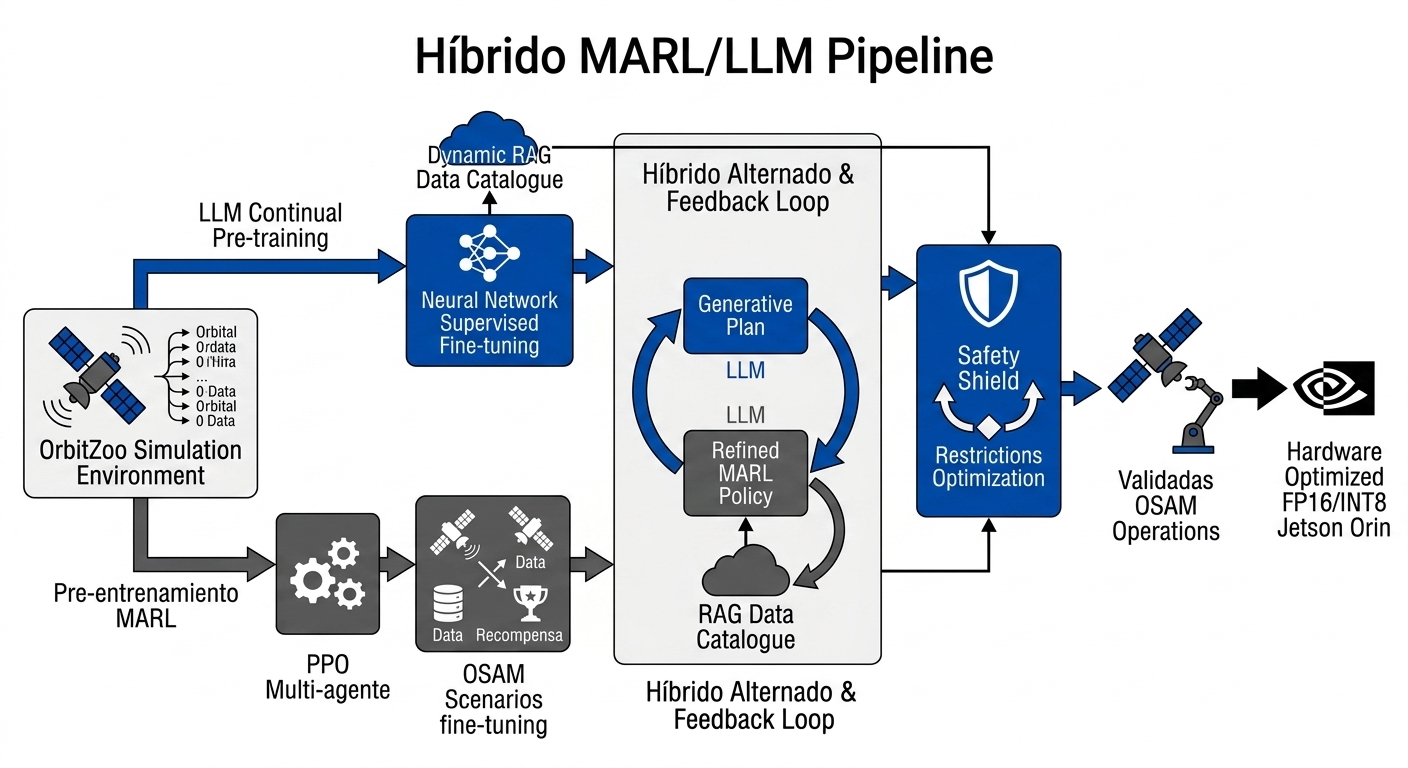
\includegraphics[width=0.95\linewidth]{fig4.png}
\caption{Pipeline de entrenamiento híbrido para agentes MARL y LLMs en el marco propuesto.}
\label{fig:training_pipeline}
\end{figure}

\subsection{Hardware Onboard y Optimización}

Uno de los desafíos persistentes al trasladar arquitecturas avanzadas al espacio radica en las severas restricciones de cómputo, potencia y radiación. 

Nuestra implementación apunta a hardware rad-hard contemporáneo, principalmente variantes de NVIDIA Jetson Orin con configuraciones de memoria y núcleos optimizadas para inferencia mixta (FP16/INT8). La optimización del modelo incluye cuantización agresiva del LLM backbone, pruning selectivo de attention heads menos críticas para tareas orbitales y destilación de conocimiento desde versiones más grandes hacia versiones livianas onboard.

Particularmente llamativo es el hecho de que la capa generativa opera con un presupuesto computacional reducido mediante prompting eficiente y caché de razonamientos previos, mientras que las políticas MARL se ejecutan en modo inferencia ultrarrápida. Esta partición inteligente permite mantener latencias de decisión por debajo de los 500\,ms incluso en escenarios de rendezvous cercanos.

\subsection{Garantías de Seguridad y Verificación}

Lejos de ser un asunto secundario, las garantías de seguridad constituyen el núcleo de cualquier sistema destinado a operaciones OSAM reales. 

Integramos mecanismos de escudo de seguridad basados en Runtime Assurance que monitorizan continuamente la salida de los agentes generativos y MARL. Cualquier plan propuesto debe satisfacer restricciones cinemáticas y de colisión codificadas como problemas de optimización convexa antes de su ejecución. En este sentido, trabajos previos en RL para servicers autónomos han demostrado la efectividad de combinar aprendizaje con reglas de seguridad explícitas \cite{Patnala2024_OOS_RL}.

\begin{table}[t]
\centering
\caption{Requisitos computacionales estimados para implementación onboard}
\label{tab:compute_requirements}
\begin{tabular}{lccc}
\hline
Componente & Memoria (GB) & Potencia (W) & Latencia Inferencia (ms) \\
\hline
LLM Agent (quantized) & 4.2 & 18 & 320 \\
MARL Policy & 1.1 & 8 & 45 \\
SCP Optimizer & 2.8 & 15 & 180 \\
Framework Completo & 8.5 & 45 & <500 \\
\hline
\end{tabular}
\end{table}

La Tabla 3 resume los requisitos computacionales validados en simulaciones de hardware-in-the-loop. Adicionalmente, implementamos verificación formal de subcomponentes críticos mediante model checking y monitoreo de invariantes temporales. 

Aunque estos mecanismos añaden overhead, representan una inversión necesaria que, en nuestra experiencia, marca la diferencia entre sistemas prometedores en simulación y arquitecturas confiables para despliegue orbital.